    
    
    
    

    

    \hypertarget{les-slices-en-python}{%
\section{Les slices en Python}\label{les-slices-en-python}}

    \hypertarget{compluxe9ment---niveau-basique}{%
\subsection{Complément - niveau
basique}\label{compluxe9ment---niveau-basique}}

    Ce support de cours reprend les notions de \emph{slicing} vues dans la
vidéo.

    Nous allons illustrer les slices sur la chaîne suivante, rappelez-vous
toutefois que ce mécanisme fonctionne avec toutes les séquences que l'on
verra plus tard, comme les listes ou les tuples.

    \begin{Verbatim}[commandchars=\\\{\},frame=single,framerule=0.3mm,rulecolor=\color{cellframecolor}]
{\color{incolor}In [{\color{incolor}1}]:} \PY{n}{chaine} \PY{o}{=} \PY{l+s+s2}{\PYZdq{}}\PY{l+s+s2}{abcdefghijklmnopqrstuvwxyz}\PY{l+s+s2}{\PYZdq{}}
        \PY{n+nb}{print}\PY{p}{(}\PY{n}{chaine}\PY{p}{)}
\end{Verbatim}


    \begin{Verbatim}[commandchars=\\\{\},frame=single,framerule=0.3mm,rulecolor=\color{cellframecolor}]
abcdefghijklmnopqrstuvwxyz
\end{Verbatim}

    \hypertarget{slice-sans-pas}{%
\subsubsection{Slice sans pas}\label{slice-sans-pas}}

    On a vu en cours qu'une slice permet de désigner toute une plage
d'éléments d'une séquence. Ainsi on peut écrire~:

    \begin{Verbatim}[commandchars=\\\{\},frame=single,framerule=0.3mm,rulecolor=\color{cellframecolor}]
{\color{incolor}In [{\color{incolor}2}]:} \PY{n}{chaine}\PY{p}{[}\PY{l+m+mi}{2}\PY{p}{:}\PY{l+m+mi}{6}\PY{p}{]}
\end{Verbatim}


\begin{Verbatim}[commandchars=\\\{\},frame=single,framerule=0.3mm,rulecolor=\color{cellframecolor}]
{\color{outcolor}Out[{\color{outcolor}2}]:} 'cdef'
\end{Verbatim}
            
    \hypertarget{conventions-de-duxe9but-et-fin}{%
\subsubsection{Conventions de début et
fin}\label{conventions-de-duxe9but-et-fin}}

    Les débutants ont parfois du mal avec les bornes. Il faut se souvenir
que~:

\begin{itemize}
\tightlist
\item
  les indices \textbf{commencent} comme toujours \textbf{à zéro}~;
\item
  le premier indice \texttt{debut} est \textbf{inclus}~;
\item
  le second indice \texttt{fin} est \textbf{exclu}~;
\item
  on obtient en tout \texttt{fin-debut} items dans le résultat.
\end{itemize}

Ainsi, ci-dessus, le résultat contient \texttt{6\ -\ 2\ =\ 4} éléments.

    Pour vous aider à vous souvenir des conventions de début et de fin,
souvenez-vous qu'on veut pouvoir facilement juxtaposer deux slices qui
ont une borne commune.

C'est-à-dire qu'avec~:

    \begin{figure}
\centering
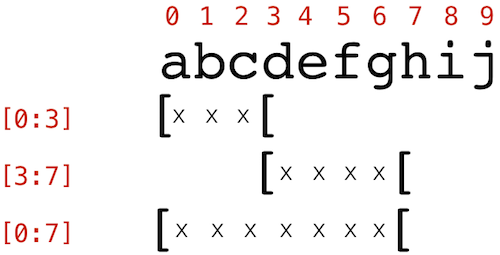
\includegraphics{media/brackets.png}
\caption{début et fin}
\end{figure}

    \begin{Verbatim}[commandchars=\\\{\},frame=single,framerule=0.3mm,rulecolor=\color{cellframecolor}]
{\color{incolor}In [{\color{incolor}3}]:} \PY{c+c1}{\PYZsh{} chaine[a:b] + chaine[b:c] == chaine[a:c]}
        \PY{n}{chaine}\PY{p}{[}\PY{l+m+mi}{0}\PY{p}{:}\PY{l+m+mi}{3}\PY{p}{]} \PY{o}{+} \PY{n}{chaine}\PY{p}{[}\PY{l+m+mi}{3}\PY{p}{:}\PY{l+m+mi}{7}\PY{p}{]} \PY{o}{==} \PY{n}{chaine}\PY{p}{[}\PY{l+m+mi}{0}\PY{p}{:}\PY{l+m+mi}{7}\PY{p}{]}
\end{Verbatim}


\begin{Verbatim}[commandchars=\\\{\},frame=single,framerule=0.3mm,rulecolor=\color{cellframecolor}]
{\color{outcolor}Out[{\color{outcolor}3}]:} True
\end{Verbatim}
            
    \hypertarget{bornes-omises}{%
\paragraph{Bornes omises}\label{bornes-omises}}

    On peut omettre une borne~:

    \begin{Verbatim}[commandchars=\\\{\},frame=single,framerule=0.3mm,rulecolor=\color{cellframecolor}]
{\color{incolor}In [{\color{incolor}4}]:} \PY{c+c1}{\PYZsh{} si on omet la première borne, cela signifie que}
        \PY{c+c1}{\PYZsh{} la slice commence au début de l\PYZsq{}objet}
        \PY{n}{chaine}\PY{p}{[}\PY{p}{:}\PY{l+m+mi}{6}\PY{p}{]}
\end{Verbatim}


\begin{Verbatim}[commandchars=\\\{\},frame=single,framerule=0.3mm,rulecolor=\color{cellframecolor}]
{\color{outcolor}Out[{\color{outcolor}4}]:} 'abcdef'
\end{Verbatim}
            
    \begin{Verbatim}[commandchars=\\\{\},frame=single,framerule=0.3mm,rulecolor=\color{cellframecolor}]
{\color{incolor}In [{\color{incolor}5}]:} \PY{c+c1}{\PYZsh{} et bien entendu c\PYZsq{}est la même chose si on omet la deuxième borne}
        \PY{n}{chaine}\PY{p}{[}\PY{l+m+mi}{24}\PY{p}{:}\PY{p}{]}
\end{Verbatim}


\begin{Verbatim}[commandchars=\\\{\},frame=single,framerule=0.3mm,rulecolor=\color{cellframecolor}]
{\color{outcolor}Out[{\color{outcolor}5}]:} 'yz'
\end{Verbatim}
            
    \begin{Verbatim}[commandchars=\\\{\},frame=single,framerule=0.3mm,rulecolor=\color{cellframecolor}]
{\color{incolor}In [{\color{incolor}6}]:} \PY{c+c1}{\PYZsh{} ou même omettre les deux bornes, auquel cas on}
        \PY{c+c1}{\PYZsh{} fait une copie de l\PYZsq{}objet \PYZhy{} on y reviendra plus tard}
        \PY{n}{chaine}\PY{p}{[}\PY{p}{:}\PY{p}{]}
\end{Verbatim}


\begin{Verbatim}[commandchars=\\\{\},frame=single,framerule=0.3mm,rulecolor=\color{cellframecolor}]
{\color{outcolor}Out[{\color{outcolor}6}]:} 'abcdefghijklmnopqrstuvwxyz'
\end{Verbatim}
            
    \hypertarget{indices-nuxe9gatifs}{%
\paragraph{Indices négatifs}\label{indices-nuxe9gatifs}}

    On peut utiliser des indices négatifs pour compter à partir de la fin~:

    \begin{Verbatim}[commandchars=\\\{\},frame=single,framerule=0.3mm,rulecolor=\color{cellframecolor}]
{\color{incolor}In [{\color{incolor}7}]:} \PY{n}{chaine}\PY{p}{[}\PY{l+m+mi}{3}\PY{p}{:}\PY{o}{\PYZhy{}}\PY{l+m+mi}{3}\PY{p}{]}
\end{Verbatim}


\begin{Verbatim}[commandchars=\\\{\},frame=single,framerule=0.3mm,rulecolor=\color{cellframecolor}]
{\color{outcolor}Out[{\color{outcolor}7}]:} 'defghijklmnopqrstuvw'
\end{Verbatim}
            
    \begin{Verbatim}[commandchars=\\\{\},frame=single,framerule=0.3mm,rulecolor=\color{cellframecolor}]
{\color{incolor}In [{\color{incolor}8}]:} \PY{n}{chaine}\PY{p}{[}\PY{o}{\PYZhy{}}\PY{l+m+mi}{3}\PY{p}{:}\PY{p}{]}
\end{Verbatim}


\begin{Verbatim}[commandchars=\\\{\},frame=single,framerule=0.3mm,rulecolor=\color{cellframecolor}]
{\color{outcolor}Out[{\color{outcolor}8}]:} 'xyz'
\end{Verbatim}
            
    \hypertarget{slice-avec-pas}{%
\subsubsection{Slice avec pas}\label{slice-avec-pas}}

    Il est également possible de préciser un \emph{pas}, de façon à ne
choisir par exemple, dans la plage donnée, qu'un élément sur deux~:

    \begin{Verbatim}[commandchars=\\\{\},frame=single,framerule=0.3mm,rulecolor=\color{cellframecolor}]
{\color{incolor}In [{\color{incolor}9}]:} \PY{c+c1}{\PYZsh{} le pas est précisé après un deuxième deux\PYZhy{}points (:)}
        \PY{c+c1}{\PYZsh{} ici on va choisir un caractère sur deux dans la plage [3:\PYZhy{}3]}
        \PY{n}{chaine}\PY{p}{[}\PY{l+m+mi}{3}\PY{p}{:}\PY{o}{\PYZhy{}}\PY{l+m+mi}{3}\PY{p}{:}\PY{l+m+mi}{2}\PY{p}{]}
\end{Verbatim}


\begin{Verbatim}[commandchars=\\\{\},frame=single,framerule=0.3mm,rulecolor=\color{cellframecolor}]
{\color{outcolor}Out[{\color{outcolor}9}]:} 'dfhjlnprtv'
\end{Verbatim}
            
    Comme on le devine, le troisième élément de la slice, ici \texttt{2},
détermine le pas. On ne retient donc, dans la chaîne \texttt{defghi...}
que \texttt{d}, puis \texttt{f}, et ainsi de suite.

On peut préciser du coup la borne de fin (ici \texttt{-3}) avec un peu
de liberté, puisqu'ici on obtiendrait un résultat identique avec
\texttt{-4}.

    \begin{Verbatim}[commandchars=\\\{\},frame=single,framerule=0.3mm,rulecolor=\color{cellframecolor}]
{\color{incolor}In [{\color{incolor}10}]:} \PY{n}{chaine}\PY{p}{[}\PY{l+m+mi}{3}\PY{p}{:}\PY{o}{\PYZhy{}}\PY{l+m+mi}{4}\PY{p}{:}\PY{l+m+mi}{2}\PY{p}{]}
\end{Verbatim}


\begin{Verbatim}[commandchars=\\\{\},frame=single,framerule=0.3mm,rulecolor=\color{cellframecolor}]
{\color{outcolor}Out[{\color{outcolor}10}]:} 'dfhjlnprtv'
\end{Verbatim}
            
    \hypertarget{pas-nuxe9gatif}{%
\subsubsection{Pas négatif}\label{pas-nuxe9gatif}}

    Il est même possible de spécifier un pas négatif. Dans ce cas, de
manière un peu contre-intuitive, il faut préciser un début (le premier
indice de la slice) qui soit \emph{plus à droite} que la fin (le second
indice).

Pour prendre un exemple, comme l'élément d'indice \texttt{-3},
c'est-à-dire \texttt{x}, est plus à droite que l'élément d'indice
\texttt{3}, c'est-à-dire \texttt{d}, évidemment si on ne précisait pas
le pas (qui revient à choisir un pas égal à \texttt{1}), on obtiendrait
une liste vide~:

    \begin{Verbatim}[commandchars=\\\{\},frame=single,framerule=0.3mm,rulecolor=\color{cellframecolor}]
{\color{incolor}In [{\color{incolor}11}]:} \PY{n}{chaine}\PY{p}{[}\PY{o}{\PYZhy{}}\PY{l+m+mi}{3}\PY{p}{:}\PY{l+m+mi}{3}\PY{p}{]}
\end{Verbatim}


\begin{Verbatim}[commandchars=\\\{\},frame=single,framerule=0.3mm,rulecolor=\color{cellframecolor}]
{\color{outcolor}Out[{\color{outcolor}11}]:} ''
\end{Verbatim}
            
    Si maintenant on précise un pas négatif, on obtient cette fois~:

    \begin{Verbatim}[commandchars=\\\{\},frame=single,framerule=0.3mm,rulecolor=\color{cellframecolor}]
{\color{incolor}In [{\color{incolor}12}]:} \PY{n}{chaine}\PY{p}{[}\PY{o}{\PYZhy{}}\PY{l+m+mi}{3}\PY{p}{:}\PY{l+m+mi}{3}\PY{p}{:}\PY{o}{\PYZhy{}}\PY{l+m+mi}{2}\PY{p}{]}
\end{Verbatim}


\begin{Verbatim}[commandchars=\\\{\},frame=single,framerule=0.3mm,rulecolor=\color{cellframecolor}]
{\color{outcolor}Out[{\color{outcolor}12}]:} 'xvtrpnljhf'
\end{Verbatim}
            
    \hypertarget{conclusion}{%
\subsubsection{Conclusion}\label{conclusion}}

    À nouveau, souvenez-vous que tous ces mécanismes fonctionnent avec de
nombreux autres types que les chaînes de caractères. En voici deux
exemples qui anticipent tous les deux sur la suite, mais qui devraient
illustrer les vastes possibilités qui sont offertes avec les slices.

    \hypertarget{listes}{%
\paragraph{Listes}\label{listes}}

    Par exemple sur les listes~:

    \begin{Verbatim}[commandchars=\\\{\},frame=single,framerule=0.3mm,rulecolor=\color{cellframecolor}]
{\color{incolor}In [{\color{incolor}13}]:} \PY{n}{liste} \PY{o}{=} \PY{p}{[}\PY{l+m+mi}{0}\PY{p}{,} \PY{l+m+mi}{2}\PY{p}{,} \PY{l+m+mi}{4}\PY{p}{,} \PY{l+m+mi}{8}\PY{p}{,} \PY{l+m+mi}{16}\PY{p}{,} \PY{l+m+mi}{32}\PY{p}{,} \PY{l+m+mi}{64}\PY{p}{,} \PY{l+m+mi}{128}\PY{p}{]}
         \PY{n}{liste}
\end{Verbatim}


\begin{Verbatim}[commandchars=\\\{\},frame=single,framerule=0.3mm,rulecolor=\color{cellframecolor}]
{\color{outcolor}Out[{\color{outcolor}13}]:} [0, 2, 4, 8, 16, 32, 64, 128]
\end{Verbatim}
            
    \begin{Verbatim}[commandchars=\\\{\},frame=single,framerule=0.3mm,rulecolor=\color{cellframecolor}]
{\color{incolor}In [{\color{incolor}14}]:} \PY{n}{liste}\PY{p}{[}\PY{o}{\PYZhy{}}\PY{l+m+mi}{1}\PY{p}{:}\PY{l+m+mi}{1}\PY{p}{:}\PY{o}{\PYZhy{}}\PY{l+m+mi}{2}\PY{p}{]}
\end{Verbatim}


\begin{Verbatim}[commandchars=\\\{\},frame=single,framerule=0.3mm,rulecolor=\color{cellframecolor}]
{\color{outcolor}Out[{\color{outcolor}14}]:} [128, 32, 8]
\end{Verbatim}
            
    Et même ceci, qui peut être déroutant. Nous reviendrons dessus.

    \begin{Verbatim}[commandchars=\\\{\},frame=single,framerule=0.3mm,rulecolor=\color{cellframecolor}]
{\color{incolor}In [{\color{incolor}15}]:} \PY{n}{liste}\PY{p}{[}\PY{l+m+mi}{2}\PY{p}{:}\PY{l+m+mi}{4}\PY{p}{]} \PY{o}{=} \PY{p}{[}\PY{l+m+mi}{100}\PY{p}{,} \PY{l+m+mi}{200}\PY{p}{,} \PY{l+m+mi}{300}\PY{p}{,} \PY{l+m+mi}{400}\PY{p}{,} \PY{l+m+mi}{500}\PY{p}{]}
         \PY{n}{liste}
\end{Verbatim}


\begin{Verbatim}[commandchars=\\\{\},frame=single,framerule=0.3mm,rulecolor=\color{cellframecolor}]
{\color{outcolor}Out[{\color{outcolor}15}]:} [0, 2, 100, 200, 300, 400, 500, 16, 32, 64, 128]
\end{Verbatim}
            
    \hypertarget{compluxe9ment---niveau-avancuxe9}{%
\subsection{Complément - niveau
avancé}\label{compluxe9ment---niveau-avancuxe9}}

    \hypertarget{numpy}{%
\paragraph{\texorpdfstring{\texttt{numpy}}{numpy}}\label{numpy}}

    La bibliothèque \texttt{numpy} permet de manipuler des tableaux ou des
matrices. En anticipant (beaucoup) sur son usage que nous reverrons bien
entendu en détail, voici un aperçu de ce que l'on peut faire avec des
slices sur des objets \texttt{numpy}~:

    \begin{Verbatim}[commandchars=\\\{\},frame=single,framerule=0.3mm,rulecolor=\color{cellframecolor}]
{\color{incolor}In [{\color{incolor}16}]:} \PY{c+c1}{\PYZsh{} ces deux premières cellules sont à admettre}
         \PY{c+c1}{\PYZsh{} on construit un tableau ligne}
         \PY{k+kn}{import} \PY{n+nn}{numpy} \PY{k}{as} \PY{n+nn}{np}
         
         \PY{n}{un\PYZus{}cinq} \PY{o}{=} \PY{n}{np}\PY{o}{.}\PY{n}{array}\PY{p}{(}\PY{p}{[}\PY{l+m+mi}{1}\PY{p}{,} \PY{l+m+mi}{2}\PY{p}{,} \PY{l+m+mi}{3}\PY{p}{,} \PY{l+m+mi}{4}\PY{p}{,} \PY{l+m+mi}{5}\PY{p}{]}\PY{p}{)}
         \PY{n}{un\PYZus{}cinq}
\end{Verbatim}


\begin{Verbatim}[commandchars=\\\{\},frame=single,framerule=0.3mm,rulecolor=\color{cellframecolor}]
{\color{outcolor}Out[{\color{outcolor}16}]:} array([1, 2, 3, 4, 5])
\end{Verbatim}
            
    \begin{Verbatim}[commandchars=\\\{\},frame=single,framerule=0.3mm,rulecolor=\color{cellframecolor}]
{\color{incolor}In [{\color{incolor}17}]:} \PY{c+c1}{\PYZsh{} ces deux premières cellules sont à admettre}
         \PY{c+c1}{\PYZsh{} on le combine avec lui\PYZhy{}même \PYZhy{} et en utilisant une slice un peu magique}
         \PY{c+c1}{\PYZsh{} pour former un tableau carré 5x5}
         
         \PY{n}{array} \PY{o}{=} \PY{l+m+mi}{10} \PY{o}{*} \PY{n}{un\PYZus{}cinq}\PY{p}{[}\PY{p}{:}\PY{p}{,} \PY{n}{np}\PY{o}{.}\PY{n}{newaxis}\PY{p}{]} \PY{o}{+} \PY{n}{un\PYZus{}cinq}
         \PY{n}{array}
\end{Verbatim}


\begin{Verbatim}[commandchars=\\\{\},frame=single,framerule=0.3mm,rulecolor=\color{cellframecolor}]
{\color{outcolor}Out[{\color{outcolor}17}]:} array([[11, 12, 13, 14, 15],
                [21, 22, 23, 24, 25],
                [31, 32, 33, 34, 35],
                [41, 42, 43, 44, 45],
                [51, 52, 53, 54, 55]])
\end{Verbatim}
            
    Sur ce tableau de taille 5x5, nous pouvons aussi faire du slicing et
extraire le sous-tableau 3x3 au centre~:

    \begin{Verbatim}[commandchars=\\\{\},frame=single,framerule=0.3mm,rulecolor=\color{cellframecolor}]
{\color{incolor}In [{\color{incolor}18}]:} \PY{n}{centre} \PY{o}{=} \PY{n}{array}\PY{p}{[}\PY{l+m+mi}{1}\PY{p}{:}\PY{l+m+mi}{4}\PY{p}{,} \PY{l+m+mi}{1}\PY{p}{:}\PY{l+m+mi}{4}\PY{p}{]}
         \PY{n}{centre}
\end{Verbatim}


\begin{Verbatim}[commandchars=\\\{\},frame=single,framerule=0.3mm,rulecolor=\color{cellframecolor}]
{\color{outcolor}Out[{\color{outcolor}18}]:} array([[22, 23, 24],
                [32, 33, 34],
                [42, 43, 44]])
\end{Verbatim}
            
    On peut bien sûr également utiliser un pas~:

    \begin{Verbatim}[commandchars=\\\{\},frame=single,framerule=0.3mm,rulecolor=\color{cellframecolor}]
{\color{incolor}In [{\color{incolor}19}]:} \PY{n}{coins} \PY{o}{=} \PY{n}{array}\PY{p}{[}\PY{p}{:}\PY{p}{:}\PY{l+m+mi}{4}\PY{p}{,} \PY{p}{:}\PY{p}{:}\PY{l+m+mi}{4}\PY{p}{]}
         \PY{n}{coins}
\end{Verbatim}


\begin{Verbatim}[commandchars=\\\{\},frame=single,framerule=0.3mm,rulecolor=\color{cellframecolor}]
{\color{outcolor}Out[{\color{outcolor}19}]:} array([[11, 15],
                [51, 55]])
\end{Verbatim}
            
    Ou bien retourner complètement dans une direction~:

    \begin{Verbatim}[commandchars=\\\{\},frame=single,framerule=0.3mm,rulecolor=\color{cellframecolor}]
{\color{incolor}In [{\color{incolor}20}]:} \PY{n}{tete\PYZus{}en\PYZus{}bas} \PY{o}{=} \PY{n}{array}\PY{p}{[}\PY{p}{:}\PY{p}{:}\PY{o}{\PYZhy{}}\PY{l+m+mi}{1}\PY{p}{,}\PY{p}{:}\PY{p}{]}
         \PY{n}{tete\PYZus{}en\PYZus{}bas}
\end{Verbatim}


\begin{Verbatim}[commandchars=\\\{\},frame=single,framerule=0.3mm,rulecolor=\color{cellframecolor}]
{\color{outcolor}Out[{\color{outcolor}20}]:} array([[51, 52, 53, 54, 55],
                [41, 42, 43, 44, 45],
                [31, 32, 33, 34, 35],
                [21, 22, 23, 24, 25],
                [11, 12, 13, 14, 15]])
\end{Verbatim}
            

    % Add a bibliography block to the postdoc
    
    
    
